\chapter{Breast Cancer Data Analysis}
A subset of the previously discussed regression methods has been used on gene methylation and expression data from breast cancer patients, aiming to explore how methylation of certain genes affects the expression of others.


\section{Molecular biology background} \label{sec:mol_bio}
This section briefly presents relevant molecular biology mechanisms related to gene expression, discussed thoroughly in \cite{setubal1997introduction}. Each cell in an organism has a number of long DNA molecules, the different sections of which contain information necessary to build specific proteins. These sections of the DNA sequence are called genes and a single gene corresponds to a protein. The beginning of each gene is marked by a promoter, which is a region of the DNA sequence that indicates there is a gene ahead. Recognition of a promoter region initiates the process called transcription, which creates a copy of the gene on an RNA molecule. The produced messenger RNA is then used by the ribosome, a cell structure devoted to protein synthesis.

DNA methylation is a process which attaches methyl groups to parts of the DNA molecule. Methylation changes to the DNA can be inherited by daughter cells in the process of cell division. Consequently, such changes have the ability to dynamically modify the function of the otherwise static DNA sequence throughout the life of an organism. Methylation can occur in the gene body or the promoter region of a gene. In case of the latter, DNA methylation represses the transcription of the gene causing it to no longer be expressed, practically turning off the gene. 


\section{Breast cancer epigenetic dataset} \label{sec:brca_data}
The publicly available gene methylation and expression data used in this project is provided by the Breast Invasive Carcinoma (TCGA-BRCA \cite{cancer2012comprehensive}) project of The Cancer Genome Atlas (TCGA). Both the gene methylation and expression data is array based and preprocessed to Level 3 in accordance with the TCGA protocols. The contained data is extracted from tissue samples for a subset of 215 patients diagnosed with breast invasive carcinoma available at the time of download, April 2015. 

Illumina Infinium Human DNA Methylation 450 is the platform used for the extraction of the gene methylation. It quantifies the levels of methylation at specific locations within the genome, denoted as probes. The set of probes is filtered to only retain those with less than $10\%$ missing values across all 215 samples. Each of the retained probes is associated with a specific gene depending on the location of the probe in the genome.
The probes associated with each gene are then separated into two subsets depending on their location in the gene sequence - located in the promoter or gene body regions (see Section \ref{sec:mol_bio}). To clarify, probes located in the TSS1500, TSS200, 5'UTR and first exon regions are associated with the promoter region of the gene, while those located in the body or the 3'UTR are mapped to the gene body.

Values for the methylation levels of the entire promoter and body regions are calculated for each gene and patient in the dataset. Methylation level of a gene region is defined as the mean methylation level of all probes mapped to the region. Two matrices are populated by these calculations, containing methylation levels for the promoter and gene body regions respectively.
Columns in the two matrices are further filtered to only include genes that are known or suspected to be related to breast cancer development. Gene associations with the disease are obtained from the HEFalMp (Human Experimental/FunctionAL MaPper) \cite{huttenhower2009exploring}. The final number of genes in the promoter and gene body methylation matrices is 468 and 479 respectively.

A matrix of gene expression levels is created for each of the two methylation matrices from data provided by the TCGA. Each expression matrix contains data for an equivalent set of genes as its corresponding methylation matrix and observations for the same subset of patients. 
For each of the two datasets, a co-expression based functional linkage gene network for the corresponding subset of genes is obtained from \cite{zhang2013network}. These gene networks, used by the network-constrained regression methods, are undirected graphs, whose nodes correspond to genes and edges represent a significant co-expression relationship between pairs of genes.

%The choice of epigenetic datasets, their preprocessing and the construction of a gene network, discussed in Section \ref{sec:brca_net}, have been carried out prior to the start of my project by Hui Xiao, PhD student in the Computer Laboratory at the University of Cambridge, and Antonella Iuliano, PhD student in the Department of Mathematics at the University of Salerno.


\section{Regression methods and setup}
A subset of the regression methods discussed in Chapter \ref{background} is selected for use on the breast cancer data. The chosen regression methods are the Lasso, Elastic Net, Grace, Linf and the proposed Composite method.
The optimal hyperparameter values discussed in Section \ref{sec:opt_param_val} have been used for preliminary calculations and are shown in Table 
9.1 % NUMBERING HACK
in the "Suggested value" column. The number of edges in the breast cancer gene networks is significantly higher than that of the generated datasets. Consequently, some of the hyperparameter values were manually tuned in order to improve the obtained results. The final set of hyperparameter values used to obtain the results presented in the following sections is shown in the "Selected value" column.

{\def\arraystretch{1.5}\tabcolsep=10pt
	\begin{table}[H]
		\label{tab:numbering_hack}
		\caption{Parameter values used for regression methods on the real datasets}
		\centering
		\begin{tabular}{l l r r}
			\hline\hline 
			Method name & Parameter name & Suggested value & Selected value\\
			\hline\hline
			Lasso	&	Alpha	&	0.1	&	0.04\\
			\hline
			Elastic Net	&	Alpha	&	0.2	&	0.04\\
						&	L1 ratio&	0.8	&	0.9\\
			\hline
			Grace	&	Lambda 1	&	10.0	&	10.0\\
					&	Lambda 2	&	10000.0	&	0.01\\
			\hline
			Linf	&	C	&	25.0	&	35.0\\
			\hline
			Composite	&	Vote Threshold	&	0.9	&	0.75\\
			\hline
		\end{tabular}
	\end{table}
}

We denote the "Gene body" and "Promoter" datasets as compound entities containing the methylation and corresponding expression matrix, along with the matching gene network. We hold out $\frac{1}{4}$ of the observations from each dataset for testing while the remaining $\frac{3}{4}$ are used for model fitting.

We aim to explore how the expression level of each gene is affected by the methylation levels of related genes. To achieve this, separate regression problems are defined, modeling each column in the expression matrix. Predictor values are obtained from the methylation matrix and the gene network is used by the network-constrained regression methods as needed. Although these regression problems are independent, they can be collectively thought as a multivariate regression problem producing a mapping, capable of estimating the vector of gene expression levels given a vector of gene methylation levels.


\section{Results}
The regression methods considered discovered relationships between methylation and expression for most of the genes, as shown in the "Resolved" and "Unresolved" columns of Table \ref{tab:map_summary}. The methylation of most genes was found to be unrelated to the expression levels of any gene, as shown in the "Influencing" and "Non-influencing" columns. These observations suggest that the expression levels of some genes are influenced more by the methylation level of other genes than their own methylation level.
\begin{table}[H]
	\begin{center}
		\caption{Summary of expression-methylation mappings for both datasets and all considered regression methods; resolved refers to the number of genes with found dependencies to the methylation of others; influencing refers to the number of genes whose methylation affects the expression of others}
		\label{tab:map_summary}
		\pgfplotstabletypeset[
		multicolumn names,
		col sep=comma,
		header=has colnames,
		display columns/0/.style={string type, column type = {l}},
		display columns/1/.style={string type, column type = {l}},
		display columns/2/.style={column type={S}, string type, column type = {|r}},
		display columns/3/.style={column type={S}, string type, column type = {r}},
		display columns/4/.style={column type={S}, string type, column type = {|r}},
		display columns/5/.style={column type={S}, string type, column type = {r}},
		every head row/.style={
			before row={\toprule}, 
			after row/.add={}{
				\midrule\midrule
			}
		},
		every last row/.style={
			after row=\bottomrule
		},
		every nth row={5}{before row=\midrule},
		]{tables/mapping_summary.csv}
	\end{center}
\end{table}

Table \ref{tab:sel_vars} shows the mean number of variables selected by each regression method for both datasets. These values are slightly lower for the promoter dataset as it contains a lower number of predictors. The Linf models consistently used a larger set of genes compared to the other models.
\begin{table}[H]
	\begin{center}
		\caption{Mean \textnumero$\ $of selected variables by regression method and dataset}
		\label{tab:sel_vars}
		\setlength{\tabcolsep}{12pt}
		\pgfplotstabletypeset[
		multicolumn names,
		col sep=comma,
		header=has colnames,
		display columns/0/.style={string type, column name = Dataset, column type = {l|}},
		display columns/1/.style={column type={S}, string type, column type = {r}},
		display columns/2/.style={column type={S}, string type, column type = {r}},
		display columns/3/.style={column type={S}, string type, column type = {r}},
		display columns/4/.style={column type={S}, string type, column type = {r}},
		display columns/5/.style={column type={S}, string type, column type = {r}},
		every head row/.style={
			before row={\toprule}, 
			after row/.add={}{
				\midrule\midrule
			}
		},
		every last row/.style={
			after row=\bottomrule
		},
		]{tables/selected_variables.csv}
	\end{center}
\end{table}
\pagebreak

The test MSE for all regression methods and both datasets is shown in Table \ref{tab:map_errors} and Figure \ref{fig:map_errors}. The scores are nearly identical both in therms of the mean MSE and its standard deviation. Similar to the results obtained from the synthetic datasets, the low mean MSE causes the standard deviation to appear especially large.

\begin{table}[H]
	\begin{center}
		\caption{Summary of the mean squared test errors for both datasets}
		\label{tab:map_errors}
		\setlength{\tabcolsep}{18pt}
		\pgfplotstabletypeset[
		multicolumn names,
		col sep=comma,
		header=has colnames,
		display columns/0/.style={string type, column type = {l}},
		display columns/1/.style={string type, column type = {l}},
		display columns/2/.style={column type={S}, string type, column type = {r}},
		display columns/3/.style={column type={S}, column name={$\sigma_{MSE}$}, string type, column type = {r}},
		every head row/.style={
			before row={\toprule}, 
			after row/.add={}{
				\midrule\midrule
			}
		},
		every last row/.style={
			after row=\bottomrule
		},
		every nth row={5}{before row=\midrule},
		]{tables/mapping_errors.csv}
	\end{center}
\end{table}
\begin{figure}[H]
	\centering
	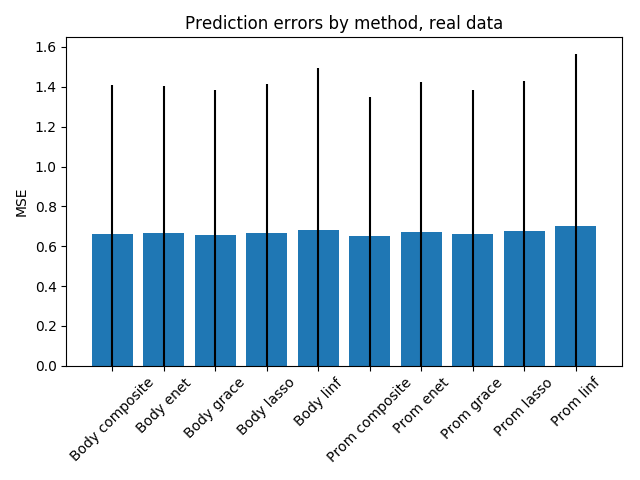
\includegraphics[scale=0.7]{mappings/errors}
	\caption{MSE by regression method and dataset}
	\label{fig:map_errors}
\end{figure}
\pagebreak


\subsection{Lasso}
Summaries of the methylation-expression mapping dependencies for the gene body and promoter datasets are shown in Figure \ref{fig:map_body_lasso} and Figure \ref{fig:map_prom_lasso} respectively.
\begin{figure}[H]
	\centering
	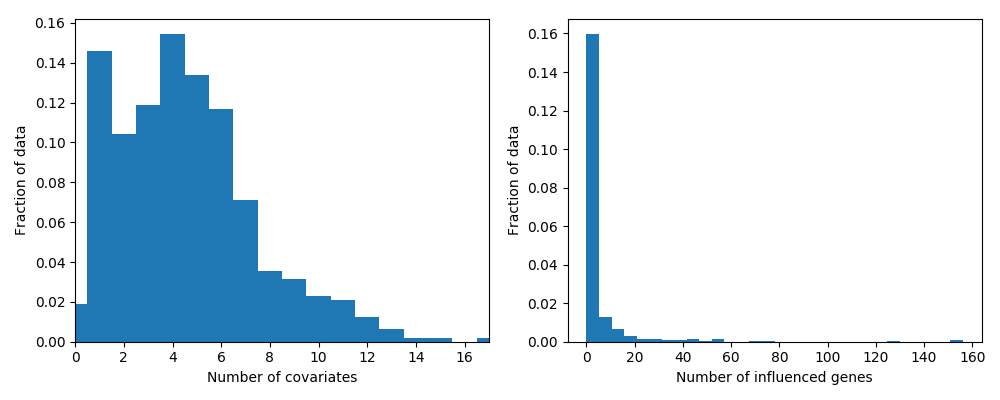
\includegraphics[scale=0.54]{mappings/distributions/Lasso_Body}
	\caption{Lasso mapping summary for gene body dataset; methylation dependencies for each gene's expression (left); genes with expression affected by each gene's methylation (right)}
	\label{fig:map_body_lasso}
\end{figure}
\begin{figure}[H]
	\centering
	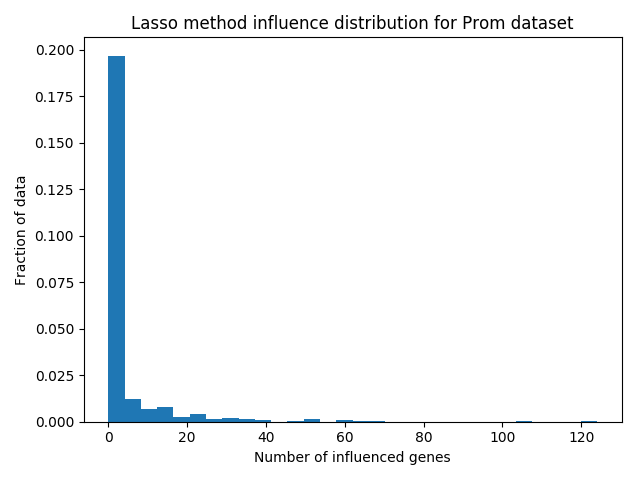
\includegraphics[scale=0.54]{mappings/distributions/Lasso_Prom}
	\caption{Lasso mapping summary for promoter dataset; methylation dependencies for each gene's expression (left); genes with expression affected by each gene's methylation (right)}
	\label{fig:map_prom_lasso}
\end{figure}
\pagebreak


\subsection{Elastic Net}
Summaries of the methylation-expression mapping dependencies for the gene body and promoter datasets are shown in Figure \ref{fig:map_body_enet} and Figure \ref{fig:map_prom_enet} respectively.
\begin{figure}[H]
	\centering
	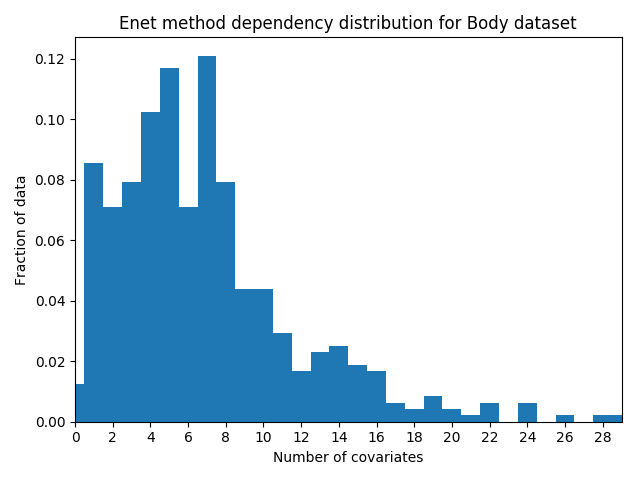
\includegraphics[scale=0.54]{mappings/distributions/Enet_Body}
	\caption{Elastic Net mapping summary for gene body dataset; methylation dependencies for each gene's expression (left); genes with expression affected by each gene's methylation (right)}
	\label{fig:map_body_enet}
\end{figure}
\begin{figure}[H]
	\centering
	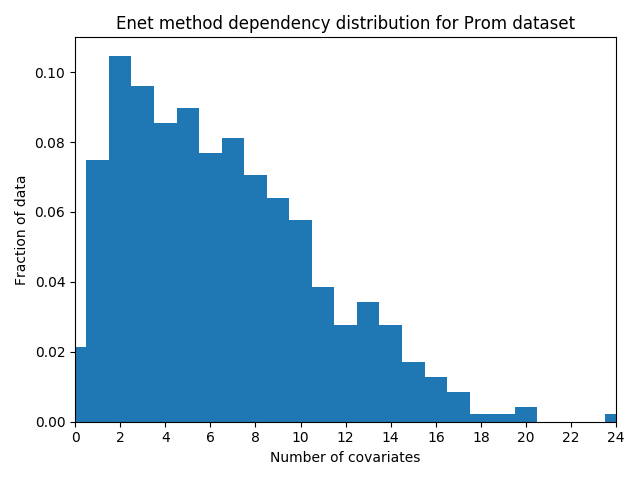
\includegraphics[scale=0.54]{mappings/distributions/Enet_Prom}
	\caption{Elastic Net mapping summary for promoter dataset; methylation dependencies for each gene's expression (left); genes with expression affected by each gene's methylation (right)}
	\label{fig:map_prom_enet}
\end{figure}
\pagebreak


\subsection{Grace}
Summaries of the methylation-expression mapping dependencies for the gene body and promoter datasets are shown in Figure \ref{fig:map_body_grace} and Figure \ref{fig:map_prom_grace} respectively.
\begin{figure}[H]
	\centering
	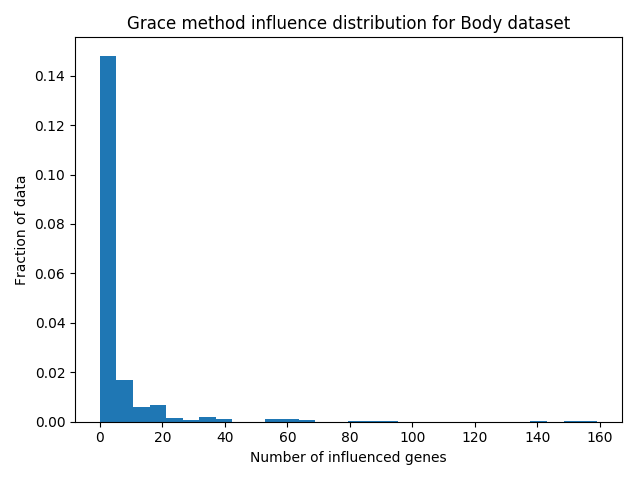
\includegraphics[scale=0.54]{mappings/distributions/Grace_Body}
	\caption{Grace mapping summary for gene body dataset; methylation dependencies for each gene's expression (left); genes with expression affected by each gene's methylation (right)}
	\label{fig:map_body_grace}
\end{figure}
\begin{figure}[H]
	\centering
	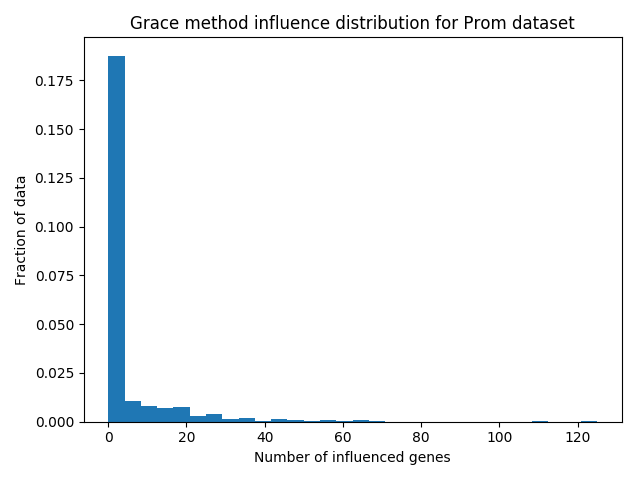
\includegraphics[scale=0.54]{mappings/distributions/Grace_Prom}
	\caption{Grace mapping summary for promoter dataset; methylation dependencies for each gene's expression (left); genes with expression affected by each gene's methylation (right)}
	\label{fig:map_prom_grace}
\end{figure}
\pagebreak


\subsection{Linf}
Summaries of the methylation-expression mapping dependencies for the gene body and promoter datasets are shown in Figure \ref{fig:map_body_linf} and Figure \ref{fig:map_prom_linf} respectively.
\begin{figure}[H]
	\centering
	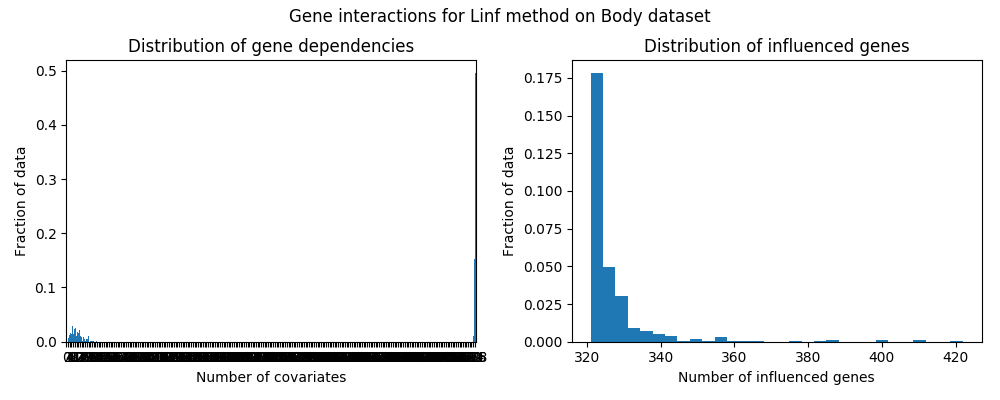
\includegraphics[scale=0.54]{mappings/distributions/Linf_Body}
	\caption{Linf mapping summary for gene body dataset; methylation dependencies for each gene's expression (left); genes with expression affected by each gene's methylation (right)}
	\label{fig:map_body_linf}
\end{figure}
\begin{figure}[H]
	\centering
	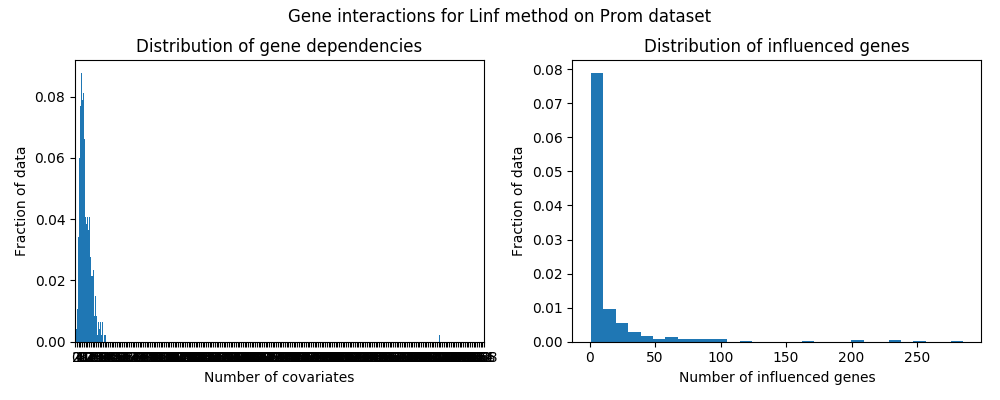
\includegraphics[scale=0.54]{mappings/distributions/Linf_Prom}
	\caption{Linf mapping summary for promoter dataset; methylation dependencies for each gene's expression (left); genes with expression affected by each gene's methylation (right)}
	\label{fig:map_prom_linf}
\end{figure}
\pagebreak


\subsection{Composite}
Summaries of the methylation-expression mapping dependencies for the gene body and promoter datasets are shown in Figure \ref{fig:map_body_comp} and Figure \ref{fig:map_prom_comp} respectively.
\begin{figure}[H]
	\centering
	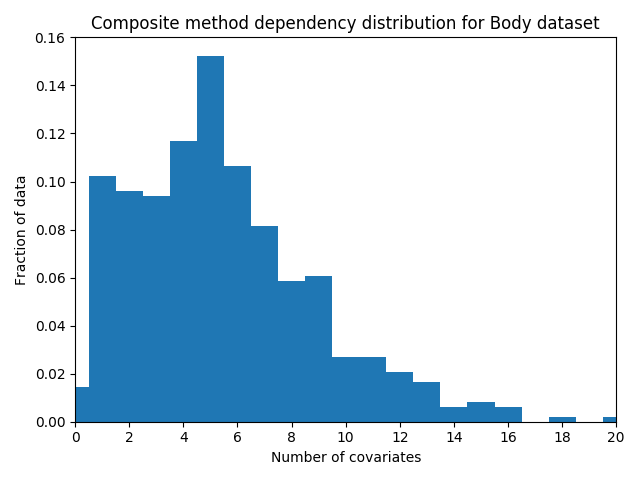
\includegraphics[scale=0.54]{mappings/distributions/Composite_Body}
	\caption{Composite method mapping summary for gene body dataset; methylation dependencies for each gene's expression (left); genes with expression affected by each gene's methylation (right)}
	\label{fig:map_body_comp}
\end{figure}
\begin{figure}[H]
	\centering
	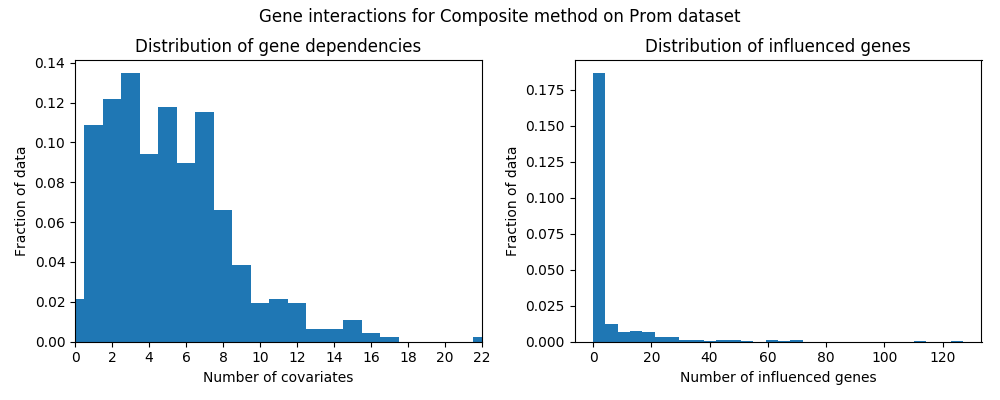
\includegraphics[scale=0.54]{mappings/distributions/Composite_Prom}
	\caption{Composite method mapping summary for promoter dataset; methylation dependencies for each gene's expression (left); genes with expression affected by each gene's methylation (right)}
	\label{fig:map_prom_comp}
\end{figure}
\pagebreak

The overall fraction of votes distribution for each gene's methylation relevance to the expression of each gene is shown in Figure \ref{fig:map_vote_dist}, note the logarithmic scale of the vertical axis. All methods are in complete agreement for the vast majority of relationships, that is in the cases where the fraction of votes is either 0 or 1. The threshold to consider a predictor relevant to the current regression problem is a vote fraction of 0.75 or higher, which describes the cases counted in the rightmost two bins in each subfigure.
\begin{figure}[H]
	\centering
	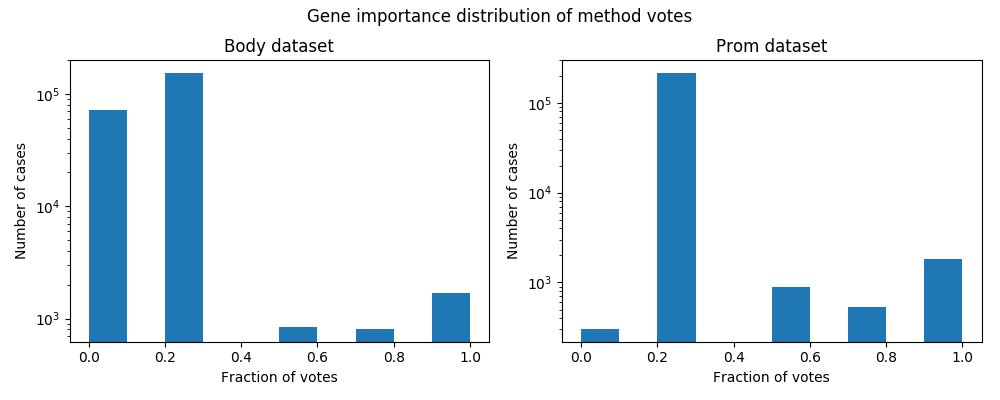
\includegraphics[scale=0.54]{mappings/vote_distribution}
	\caption{Predictor importance fraction of votes distribution for gene body (left) and promoter (right) datasets}
	\label{fig:map_vote_dist}
\end{figure}


\section{Discussion}
The methylation-expression relationship mappings produced by the various regression methods are very similar with the exception of the Linf method which consistently selected a larger subset of the genes. The expression level of most genes is affected by the methylation of a small subset of no more than 30 genes. 

A few of the genes appear to be greatly influential, namely ARHGAP11A, GPSM2 and ODF1 for the gene body dataset and DSG1 and FUT3 for the promoter dataset. The methylation level of each is found to affect the expression levels of over 100 genes.
\pagebreak


\section{Supplementary digital materials}
A digital copy of this report, CSV files of the datasets used, coefficient estimates of the methylation-expression mapping, detailed results from all conducted experiments, complete source code and full-sized figures can be requested by email sivodaskalov@gmail.com